\documentclass[a4paper]{article}
\usepackage[utf8]{inputenc}
\usepackage{graphicx}
\graphicspath{ {imgs/} }
\usepackage{floatrow}
\usepackage{array}
\usepackage[margin=1in]{geometry}
\usepackage{courier}
\usepackage{etoolbox}
\usepackage[htt]{hyphenat}
\usepackage[dvipsnames,table]{xcolor}
\usepackage{listings}
\usepackage{makecell}

\usepackage{hyperref}
\hypersetup{
    colorlinks=true,
    linkcolor=blue,
    filecolor=magenta,      
    urlcolor=cyan,
}

\renewcommand\theadalign{bc}
\renewcommand\theadfont{\bfseries}
\renewcommand\theadgape{\Gape[4pt]}
\renewcommand\cellgape{\Gape[4pt]}
\definecolor{codegreen}{rgb}{0,0.6,0}
\definecolor{codegray}{rgb}{0.5,0.5,0.5}
\definecolor{codepurple}{rgb}{0.58,0,0.82}
\definecolor{backcolour}{rgb}{0.95,0.95,0.92}

\lstdefinestyle{mystyle}{
    backgroundcolor=\color{backcolour},   
    commentstyle=\color{codegreen},
    keywordstyle=\color{magenta},
    numberstyle=\tiny\color{codegray},
    stringstyle=\color{codepurple},
    basicstyle=\ttfamily\footnotesize,
    breakatwhitespace=false,         
    breaklines=true,                 
    captionpos=b,                    
    keepspaces=true,                 
    numbers=left,                    
    numbersep=5pt,                  
    showspaces=false,                
    showstringspaces=false,
    showtabs=false,                  
    tabsize=2
}

\lstset{style=mystyle}

\title{\textbf{GIT Department Of Computer Engineering\\ 
CSE 222/505 - Spring 2020\\
Homework 4 Report \vspace{1in}}}

\author{\textbf{Fatih Kaan Salgır} \\ 
\textbf{171044009}}

\date{}

\begin{document}

\begin{large}

  \maketitle

  \newpage

  \begin{center}
    \textbf{ \\
      \vspace{3cm}
      \Huge{PART 2}
    }
  \end{center}

  \newpage


  \section{Problem Solution Approach}

  The assignment is implementing a \texttt{Deque<E>} class. I have started by reading \href{https://docs.oracle.com/javase/7/docs/api/java/util/Deque.html}{'Deque javadoc'} of Oracle. Thus I had enough knowledge about method signatures, what they return and whether they throw exception or not.

  \vspace{1em}
  I preferred to keep 2 \texttt{LinkedList}s in \texttt{Deque}, so that I can avoid code repetition for operations on deque and removed nodes.

  \vspace{1em}
  To implement \texttt{iterator} and \texttt{descendingIterator} I created new inner classes, and I have filled necessary methods which are \texttt{next()} and \texttt{hasNext()}. For \texttt{remove()} method I have preferred to throw  \texttt{UnsupportedOperationException}, unless \\\texttt{lastReturned} node is either first or last node.

  \newpage



  \section{Class Diagrams}


  \begin{figure}[htp]
    \centering
    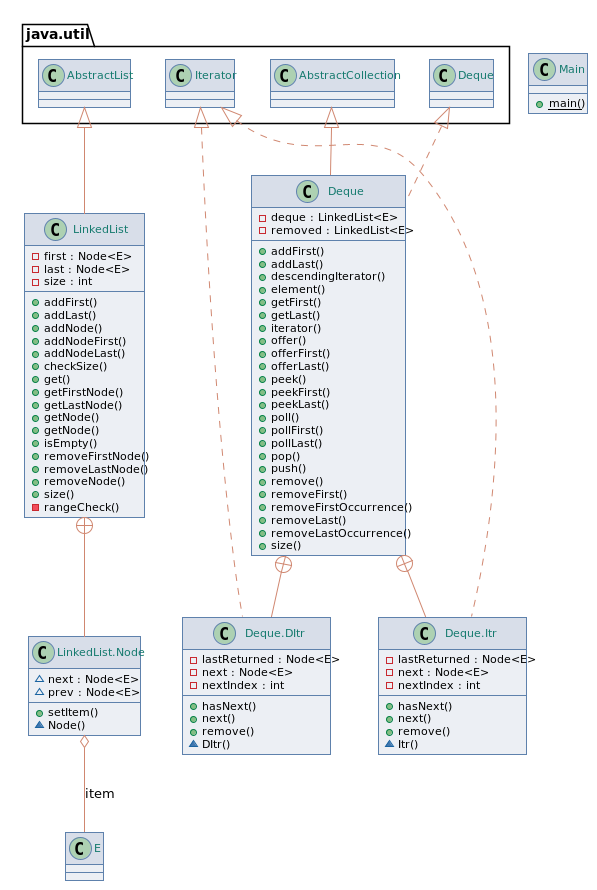
\includegraphics[width=0.8\textwidth]{class-diagram}
  \end{figure}

  \newpage


  \section{Test Cases}

  I have created some text cases for some adding and removing operations which is present on my main method.

  \begin{center}
    \begin{table}[htp]
      \rowcolors{1}{black!5}{gray!5}
      \begin{tabular}{ |m{1cm}|m{3cm}|p{3cm}|m{6em}|m{6em}|m{2cm}|l|  }
        \hline
        \rowcolor{RoyalBlue!30}
        \thead{Test                                                                                                                                                \\ Case \\ ID} & \thead{Test \\ Scenario} & \thead{Test Steps} &\thead{Expected \\ Results} & \thead{Actual \\ Results} & \thead{Pass/Fail}\\
        \hline
        \makecell{T01} & \makecell[lb]{add new element                                                                                                             \\with various \\methods} & \makecell[l]{1. deque.addFirst(2)\\ 2. deque.push(1) \\3. deque.offer(3)\\ 4. deque.addLast(4)} & \makecell{[1,2,3,4]} & \makecell{As expected} & \makecell{Pass}  \\ \hline
        \makecell{T02} & \makecell[lb]{iterate through                                                                                                             \\deque and print} & \makecell[l]{while iterator has \\next, iteratate and \\print} & \makecell{1 2 3 4} & \makecell{As expected} & \makecell{Pass}  \\ \hline
        \makecell{T03} & \makecell[lb]{iterate through                                                                                                             \\ deque reversely \\ and print}& \makecell[l]{while descending \\iterator has next,\\ iteratate and print} & \makecell{4 3 2 1} & \makecell{As expected} & \makecell{Pass}  \\ \hline
        \makecell{T04} & \makecell[b]{remove first element} & \makecell[l]{deque.removeFirst()} & \makecell{[2,3,4]}    & \makecell{As expected} & \makecell{Pass} \\ \hline
        \makecell{T05} & \makecell[b]{remove last element}  & \makecell[l]{deque.removeLast()}  & \makecell{[2,3]}      & \makecell{As expected} & \makecell{Pass} \\ \hline
        \makecell{T06} & \makecell[lb]{peek first element}  & \makecell[l]{deque.peekFirst()}   & \makecell{2}          & \makecell{As expected} & \makecell{Pass} \\ \hline
        \makecell{T07} & \makecell[lb]{poll from deque}     & \makecell[l]{deque.poll()}        & \makecell{deque: [3]} & \makecell{As expected} & \makecell{Pass} \\ \hline
        \makecell{T08} & \makecell[lb]{pop from deque}      & \makecell[l]{deque.pop()}         & \makecell{deque: []                                              \\ (empty)} & \makecell{As expected} & \makecell{Pass}  \\ \hline
        \makecell{T09} & \makecell[lb]{poll from deque,                                                                                                            \\ when is empty} & \makecell[l]{deque.poll()} & \makecell{returns null} & \makecell{As expected} & \makecell{Pass}  \\ \hline
        \makecell{T10} & \makecell[l]{pop from deque,                                                                                                              \\ when is empty } & \makecell[l]{deque.pop()}  & \makecell{Throw \\ exception} & \makecell{As expected} & \makecell{Pass}  \\ \hline
      \end{tabular}

    \end{table}

  \end{center}



  \newpage

  \section{Running and Results}

  \begin{lstlisting}[language=Java, caption=Testing methods in main method]
Deque<Integer> deque = new Deque<>();
System.out.println("Test Cases");
System.out.println("T01");
deque.addFirst(2);
deque.push(1);

deque.offer(3);
deque.addLast(4);

System.out.println(deque);

System.out.println("T02");
Iterator<Integer> iter = deque.iterator();
while (iter.hasNext())
  System.out.print(iter.next() + " ");
System.out.println();

System.out.println("T03");
Iterator<Integer> diter = deque.descendingIterator();
while (diter.hasNext())
  System.out.print(diter.next() + " ");
System.out.println();

System.out.println("T04");
deque.removeFirst();
System.out.println(deque);

System.out.println("T05");
deque.removeLast();
System.out.println(deque);

System.out.println("T06");
System.out.println(deque.peekFirst());
System.out.println(deque);

System.out.println("T07");
deque.poll();
System.out.println(deque);

System.out.println("T08");
deque.pop();
System.out.println(deque);

System.out.println("T09");
System.out.println(deque.poll());
System.out.println(deque);

System.out.println("T10");
deque.pop();
System.out.println(deque);
    
\end{lstlisting}

  \newpage

  Output of the test cases;

  \begin{small}
    \begin{verbatim}
Test Cases
T01
[1, 2, 3, 4]
T02
1 2 3 4 
T03
4 3 2 1 
T04
[2, 3, 4]
T05
[2, 3]
T06
2
[2, 3]
T07
[3]
T08
[]
T09
null
[]
T10
Exception in thread "main" java.util.NoSuchElementException: stack is empty
	at LinkedList.checkSize(LinkedList.java:10)
	at Deque.removeFirst(Deque.java:150)
	at Deque.pop(Deque.java:260)
	at Main.main(Main.java:53)
\end{verbatim}
  \end{small}

  \newpage

  \begin{center}
    \textbf{ \\
      \vspace{3cm}
      \Huge{PART 3}
    }
  \end{center}

  \newpage

  \setcounter{section}{0}

  \section{Problem Solution Approach}

  I have created a public static method for every problem, and since I need some extra parameters, I have called private helper methods. 

  \begin{enumerate}
    \item Base case is if there is not any space in the string. In that case it will return.\\
    Otherwise append the last word to \texttt{StringBuilder} and call the method again with excluding the last word.

    \item Base case is if length of the string is greater than 0. In that case it should return if the word is elfish.\\
    Other cases are checking if current character is one of elf letters or not.\\
    At last, call the method again with substring includes rest of the characters.

    \item Base case is checking if we reach the end of the array. In that case we should return.\\
    Other case is after iterating the array once. At this point we supposed to be found the minimum element. In that case we should do the swap and find the next minimum element in rest of the array by calling the method again.\\
    Another case is while iterating the array, if there is any element less than suppositional minimum element, then update minimum element.\\
    To apply this for all elements, we call recursively this method, with next element.

    \item Base case is checking if index is less than 0, since the iteration starts from end, and goes to beginning. In this case it will return the remaining element in the stack.\\
    Other cases are if the current element is an operator or an operand. If it is operator it takes 2 operand from the stack, perform the required operation and push the result to the stack. If its operand then it will push it to the stack. Finally, call the function recursively, for previous indexes.

    \item Base case is checking if index is greater than array length, since the iteration starts from beginning, and goes to end. In this case it will return the remaining element in the stack.\\
    Other cases are if the current element is an operator or an operand. If it is operator it takes 2 operand from the stack, perform the required operation and push the result to the stack. If its operand then it will push it to the stack. Finally, call the function recursively, for previous indexes.

    \item Base case is checking if number of iterations reach the size of the array ($m \times n$). In this case it will return.\\
    Other cases are checking the direction of iteration. While iterating through the direction, if we reach the edges of the 2 dimensional array, we change the direction to the right, and update the bounds. Therefore, we reach center of the array by following the spiral path.

  \end{enumerate}

  \newpage

  \section{Class Diagram}

  \begin{figure}[htp]
    \centering
    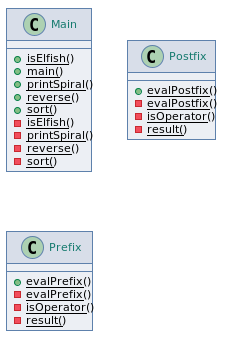
\includegraphics[width=0.4\textwidth]{class-diagram-2}
  \end{figure}

  
  \newpage

  \section{Test Cases}

  I tested methods in my main method.
  
  \begin{lstlisting}[language=Java, caption=Testing methods in main method]
    System.out.println("Test Cases");
    System.out.println("T_1.1");
    System.out.println(reverse("this function writes the sentence in reverse"));
    System.out.println("T_1.2");
    System.out.println(reverse("oneWord"));
    System.out.println("T_1.3");
    System.out.println(reverse("")); //empty string

    System.out.println("T_2.1");
    System.out.println(isElfish("white leaf"));
    System.out.println("T_2.2");
    System.out.println(isElfish("not ELFish"));
    System.out.println("T_2.3");
    System.out.println(isElfish("")); //empty string

    int[] arr = {3, 5, 7, 1, 2, 4, 9, 8, 6, 0};
    int[] emptyArr = {};

    System.out.println("T_3.1");
    sort(arr);
    for (int value : arr)
      System.out.print(value + " ");
    System.out.println();

    System.out.println("T_3.2");
    sort(emptyArr);

    System.out.println("T_4.1");
    System.out.println(Postfix.evalPostfix("3 4 1 2 * - 2 / + 5 + 6 3 / -"));
    System.out.println("T_4.2");
    System.out.println(Postfix.evalPostfix(""));
    System.out.println("T_5.1");
    System.out.println(Prefix.evalPrefix("- + + 3 / - 4 * 1 2 2 5 / 6 3"));
    System.out.println("T_5.2");
    System.out.println(Prefix.evalPrefix(""));

    System.out.println("T_6.1");
    int[][] arr2D = {{1, 2, 3, 4}, {5, 6, 7, 8}, {9, 10, 11, 12}, {13, 14, 15, 16}, {17, 18, 19, 20}};
    int[][] emptyArr2D = new int[][]{};

    printSpiral(arr2D);
    System.out.println("T_6.2");
    printSpiral(emptyArr2D);
  \end{lstlisting}

  \newpage

  Here's the result;

  \begin{small}
    \begin{verbatim}
Test Cases
T_1.1
reverse in sentence the writes function
T_1.2
oneWord
T_1.3

T_2.1
true
T_2.2
false
T_2.3
false
T_3.1
0 1 2 3 4 5 6 7 8 9 
T_3.2
T_4.1
7.0
T_4.2
null
T_5.1
7.0
T_5.2
null
T_6.1
1 2 3 4 8 12 16 20 19 18 17 13 9 5 6 7 11 15 14 10 
T_6.2

    \end{verbatim}
  \end{small}
  




\end{large}
\end{document}

